\documentclass{article}\usepackage[]{graphicx}\usepackage[]{color}
%% maxwidth is the original width if it is less than linewidth
%% otherwise use linewidth (to make sure the graphics do not exceed the margin)
\makeatletter
\def\maxwidth{ %
  \ifdim\Gin@nat@width>\linewidth
    \linewidth
  \else
    \Gin@nat@width
  \fi
}
\makeatother

\definecolor{fgcolor}{rgb}{0.345, 0.345, 0.345}
\newcommand{\hlnum}[1]{\textcolor[rgb]{0.686,0.059,0.569}{#1}}%
\newcommand{\hlstr}[1]{\textcolor[rgb]{0.192,0.494,0.8}{#1}}%
\newcommand{\hlcom}[1]{\textcolor[rgb]{0.678,0.584,0.686}{\textit{#1}}}%
\newcommand{\hlopt}[1]{\textcolor[rgb]{0,0,0}{#1}}%
\newcommand{\hlstd}[1]{\textcolor[rgb]{0.345,0.345,0.345}{#1}}%
\newcommand{\hlkwa}[1]{\textcolor[rgb]{0.161,0.373,0.58}{\textbf{#1}}}%
\newcommand{\hlkwb}[1]{\textcolor[rgb]{0.69,0.353,0.396}{#1}}%
\newcommand{\hlkwc}[1]{\textcolor[rgb]{0.333,0.667,0.333}{#1}}%
\newcommand{\hlkwd}[1]{\textcolor[rgb]{0.737,0.353,0.396}{\textbf{#1}}}%

\usepackage{framed}
\makeatletter
\newenvironment{kframe}{%
 \def\at@end@of@kframe{}%
 \ifinner\ifhmode%
  \def\at@end@of@kframe{\end{minipage}}%
  \begin{minipage}{\columnwidth}%
 \fi\fi%
 \def\FrameCommand##1{\hskip\@totalleftmargin \hskip-\fboxsep
 \colorbox{shadecolor}{##1}\hskip-\fboxsep
     % There is no \\@totalrightmargin, so:
     \hskip-\linewidth \hskip-\@totalleftmargin \hskip\columnwidth}%
 \MakeFramed {\advance\hsize-\width
   \@totalleftmargin\z@ \linewidth\hsize
   \@setminipage}}%
 {\par\unskip\endMakeFramed%
 \at@end@of@kframe}
\makeatother

\definecolor{shadecolor}{rgb}{.97, .97, .97}
\definecolor{messagecolor}{rgb}{0, 0, 0}
\definecolor{warningcolor}{rgb}{1, 0, 1}
\definecolor{errorcolor}{rgb}{1, 0, 0}
\newenvironment{knitrout}{}{} % an empty environment to be redefined in TeX

\usepackage{alltt}
\usepackage{geometry}
\geometry{verbose,tmargin=2cm,bmargin=2cm,lmargin=2.5cm,rmargin=2.5cm}
\IfFileExists{upquote.sty}{\usepackage{upquote}}{}
\begin{document}





\title{WA State HIV Testing Histories - Description of Analysis Sample}
\author{Martina Morris and Jeanette Birnbaum}
\maketitle

\section{Sample Reminder}

\begin{itemize}
    \item N = 4943
    \item Years = 2005 to 2014
    \item everHadNegTest = TRUE for 2150 (43.5\%), FALSE for 606 (12.26\%), and NA for 2187 (44.24\%)
\end{itemize}








\section{Base Case and Upper Bound, Minimal Imputation}

\begin{knitrout}\footnotesize
\definecolor{shadecolor}{rgb}{0.969, 0.969, 0.969}\color{fgcolor}\begin{kframe}
\begin{verbatim}
##                           var    Min. 1st Qu. Median   Mean 3rd Qu.   Max.
## 1               # Diagnosed     45.00   121.5  131.0  130.1   141.8  164.0
## 2     Incidence (Base Case)     95.13   112.7  128.0  123.3   136.1  139.3
## 3   Incidence (Upper Bound)     91.71   104.4  120.4  117.2   130.8  135.9
## 4   Undiagnosed (Base Case)   1209.00  1380.0 1473.0 1426.0  1504.0 1527.0
## 5 Undiagnosed (Upper Bound)   2456.00  2686.0 2866.0 2803.0  2952.0 3002.0
\end{verbatim}
\end{kframe}

{\centering 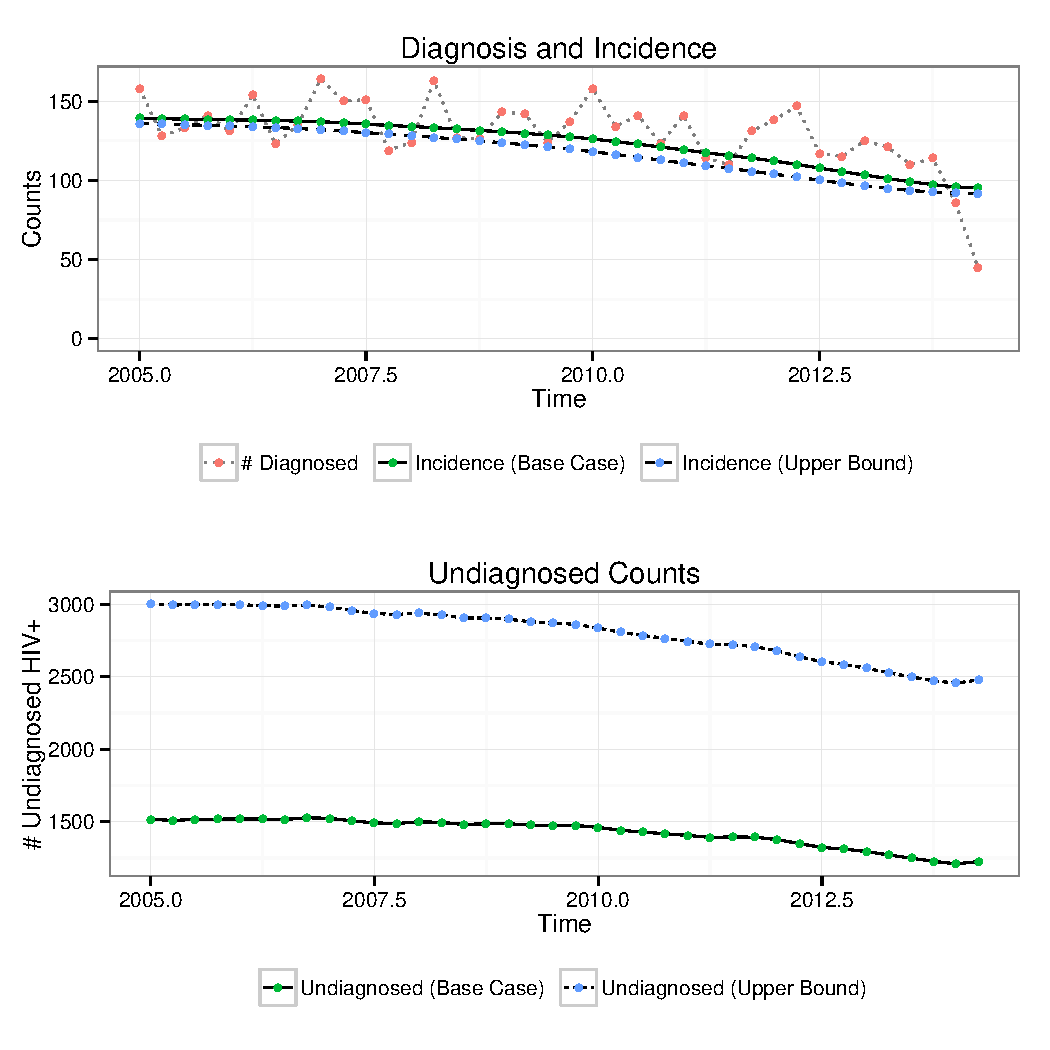
\includegraphics[width=\maxwidth]{figure/minimal-noimpute} 

}



\end{knitrout}


\section{Base Case and Upper Bound, Full Imputation}

\begin{knitrout}\footnotesize
\definecolor{shadecolor}{rgb}{0.969, 0.969, 0.969}\color{fgcolor}\begin{kframe}
\begin{verbatim}
##                           var    Min. 1st Qu. Median   Mean 3rd Qu.   Max.
## 1               # Diagnosed     45.00  121.50  131.0  130.1   141.8  164.0
## 2     Incidence (Base Case)     90.80  103.60  118.4  115.7   128.7  134.6
## 3   Incidence (Upper Bound)     87.54   95.12  105.9  104.5   114.0  119.3
## 4   Undiagnosed (Base Case)   2213.00 2438.00 2632.0 2577.0  2742.0 2816.0
## 5 Undiagnosed (Upper Bound)   4253.00 4521.00 4816.0 4782.0  5055.0 5269.0
\end{verbatim}
\end{kframe}

{\centering 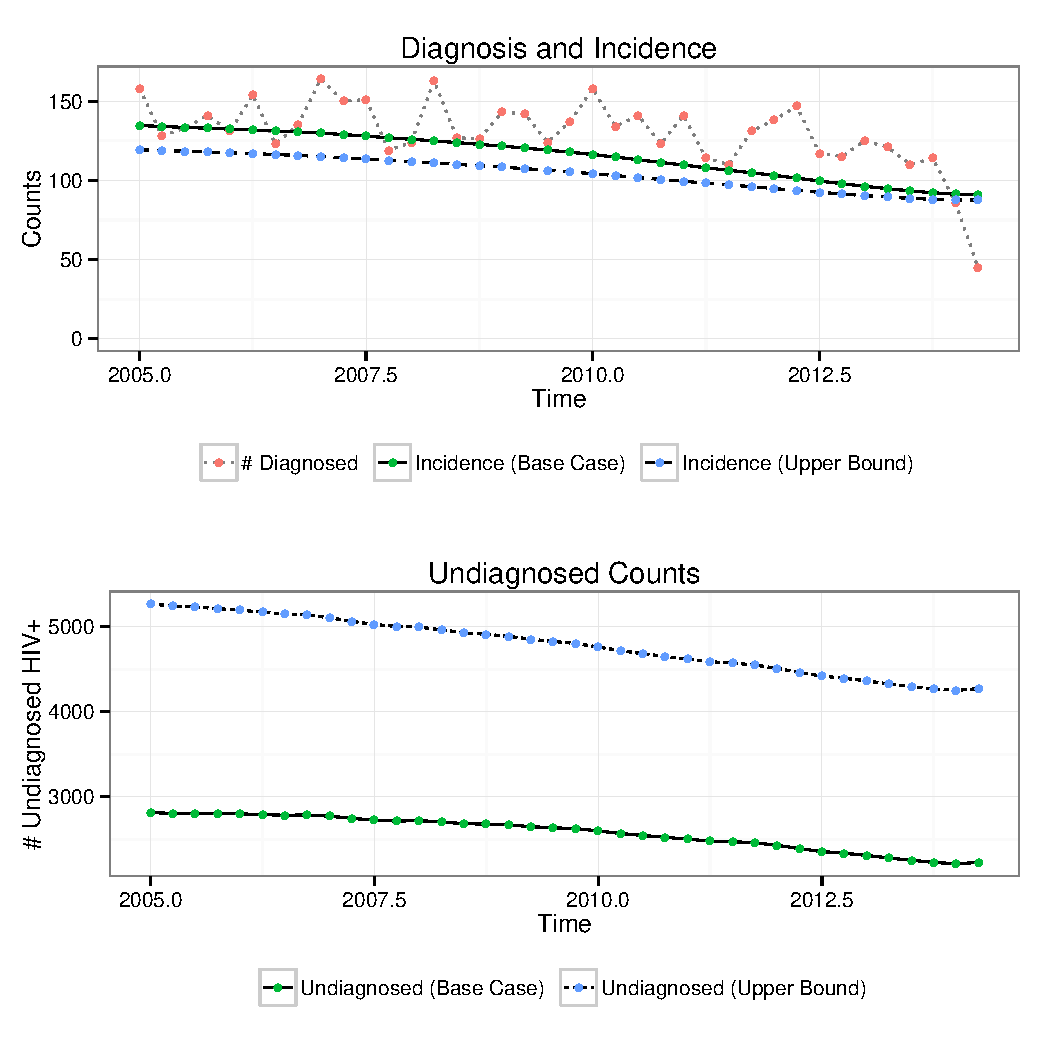
\includegraphics[width=\maxwidth]{figure/minimal-impute} 

}



\end{knitrout}


\section{Combined Results}


\begin{knitrout}\footnotesize
\definecolor{shadecolor}{rgb}{0.969, 0.969, 0.969}\color{fgcolor}\begin{kframe}
\begin{verbatim}
##    imputed                         var    Min. X1st.Qu. Median   Mean X3rd.Qu.
## 1      Yes               # Diagnosed     45.00   121.50  131.0  130.1    141.8
## 2      Yes     Incidence (Base Case)     90.80   103.60  118.4  115.7    128.7
## 3      Yes   Incidence (Upper Bound)     87.54    95.12  105.9  104.5    114.0
## 4      Yes   Undiagnosed (Base Case)   2213.00  2438.00 2632.0 2577.0   2742.0
## 5      Yes Undiagnosed (Upper Bound)   4253.00  4521.00 4816.0 4782.0   5055.0
## 6       No               # Diagnosed     45.00   121.50  131.0  130.1    141.8
## 7       No     Incidence (Base Case)     95.13   112.70  128.0  123.3    136.1
## 8       No   Incidence (Upper Bound)     91.71   104.40  120.4  117.2    130.8
## 9       No   Undiagnosed (Base Case)   1209.00  1380.00 1473.0 1426.0   1504.0
## 10      No Undiagnosed (Upper Bound)   2456.00  2686.00 2866.0 2803.0   2952.0
##      Max.
## 1   164.0
## 2   134.6
## 3   119.3
## 4  2816.0
## 5  5269.0
## 6   164.0
## 7   139.3
## 8   135.9
## 9  1527.0
## 10 3002.0
\end{verbatim}
\end{kframe}
\end{knitrout}




\end{document}


